\chapter{Introduction}
The release of advanced technologies is one of the main reasons for the revolution in various scientific research fields. In Biological and Medical domain, modern technologies are making it not only easier but also more economical than ever to undertake experiments and creating applications. As a consequence, a vast amount of biological data in terms of volume and type is generated through scientific experiments, published literature, high-throughput experiment technology, and computational analysis. This huge quantity of data are saved as biological datasets and made discoverable through web browsers, application programming interfaces, scalable search technology and extensive cross-referencing between databases. Biological databases normally contain information about gene function, structure, localization, clinical effects of mutations and similarities of biological sequences and structures.

The abundance of biological data, on the one hand, creates a golden chance for biologists to extract useful information. However, it, on the other hand, poses the challenge for scientists to wisely and effectively extract knowledge from such amount of data that normally cannot be done without the help of automated learning systems. Hence, the task of developing high performance learning systems, which help sciencists to form and assess hypotheses, plays an important role in the development of biology and medicine.
\section{Why graph-based biological data integration?}
Biological knowledge is distributed among general and specialized sources, such as gene expression, protein interaction, gene ontology, etc. It is common that information of a biological phenomenon is encoded over various heterogeneous sources. Each source captures different aspects of the phenomenon. The distribution of information over sources provides us an unprecedented opportunity to understand the phenomenon from multiple angles. Therefore, the idea of data integration which allows multiple sources of information to be treated in a unified way is potential to improve the performance of biological learning systems. Despite the fact that data integration is a promising solution, it exposes a challenge for machine learning experts and data scientists to find out optimal solutions for combining multiple sources in a big space of solutions.

\begin{figure}
\centering
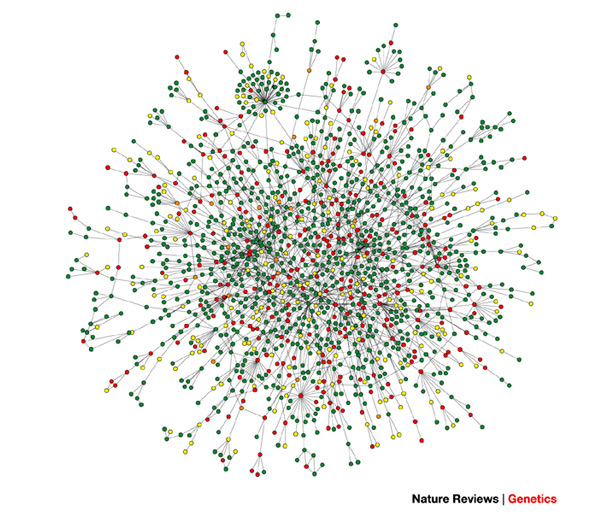
\includegraphics[width=.9\textwidth]{img/protein_interaction_net}
\caption{Yeast protein interaction network}
\label{fig:protein-interaction-net}
\end{figure}

Relations between entities encoded in biological sources can be naturally represented in form of graphs (networks) whose vertices describe for biological entities and links characterize the relations between entities. An example is the protein-protein interaction network \cref{fig:protein-interaction-net} where each vertex represents for a protein and a link connecting two vertices if they interact. Graph theory provides a mathematical abstraction for the description of such relationships. Thus, using graphs to represent for biological data allows us to \textit{i}) access to a principled and solid mathematical framework built for graphs that most scientists are familiar, \textit{ii}) develop concepts and tools which are independent of the concrete applications. By using graph presentation, the problem of biological data integration now can be converted into graph-based data integration. The final representation of data obtained by an optimal integration way is used as the input to construct inference systems (graph-based learning systems).

\section{Kernel methods for graph-based data integration and challenges}
Recently, \textit{kernel methods} whose best known member is support vector machine (SVM) \cite{cortes1995support}, has emerged as one of the most famous and powerful frameworks in machine learning. Kernel methods with the use of kernels allow to decouple the representation of the data (via kernel function) from the specific learning algorithm. Kernel representation is flexible and efficient and it provides a principled framework that allows universal type of data to be represented, including images, graphs, vectors, strings, etc. As a consequence, kernel methods are a reasonable and logical choice for graph-based inference systems. However, there are a number of challenges need to be efficiently solved, if we desire to have high performance graph-based data integration learning systems. Following are the main challenges.
\subsection{Definition of node similarity measure}
In machine learning, one of the main factors which impacts on the performance of learning systems is the definition of example similarity measure. In our context, large-scale graph-based inference systems, examples are nodes of graphs. Hence, it is necessary to have a good definition of node similarity measure. Node similarity are normally measured by \textit{graph node kernels}. However, there is not a clear way to define a graph node kernel which is efficiently applied to a wide range of graphs.
\subsection{Sparsity}
The input of a graph-based data integration system is a set of graphs which often contain sparse graphs whose number of present links are much less comparing number of actually links, due to the lack of information. For instance, in disease gene network, links connecting genes are formed when genes are involved in same diseases. New genes associated to a certain disease could be discovered over time. It means that new links could be added into networks from time to time. At a give time, a number of links discovered can be very limited, so it causes the sparsity problem. When working with sparse graphs, systems cannot effectively learn since they have access to a limited information. As a consequence, an effective solution helps to overcome the sparsity problem is crucial and needs to be proposed at hand.
\subsection{Scalability}
Given an adopted learning algorithm, the complexity of a large-scale graph-based data integration learning system incurs with the growth of the input graph set. In other words, the complexity of a graph-based learning system strongly depends on the size and the number of graphs used as its input. It is often that the complexity of a graph-based system changes at a fast pace, sometimes it exponentially changes, with respect to the cardinality of the input graph set. Therefore, scalability is an important property that a graph-based learning system is supposed to possess. It allows systems to run in reasonable time and with a reasonable memory consumption.
\subsection{Data integration methods}
Information encoded in multiple sources (graphs) provides a complementary views of phenomenon of interest. Combination information from collective sources helps to form a complete picture of the phenomenon or problem. However, optimal ways of integration are resided on a big space of solutions. Therefore, we need an effective approach to search for the optimal solutions which lead to high performance of graph-based data integration learning systems.
\section{Contributions}
The contributions of this thesis focus on solutions to overcome the challenges faced when working with large-scale graph-based biological data integration.\\

In the first contribution, we take the problem of defining node similarity measure into account by introducing an effective graph node kernel named conjunctive disjunctive node kernel (CDNK). Most existing graph node kernels are based on a notion of information diffusion which can be applied to dense
networks with high value of average node degrees. However, a drawback of these approaches is their relatively low discriminative capacity. This is in part due to the fact that information is processed in an additive and independent fashion which prevents them from accurately modeling the configuration of each gene’s context. To address this issue, we propose to employ a decompositional graph kernel technique in which the similarity function between graphs can be
formed by decomposing each graph into subgraphs and by devising a valid local
kernel between the subgraphs. To exploit its higher discriminative capacity we
first decompose the network into a collection of connected sparse graphs and then we develop a suitable kernel, CDNK.\\

The second contribution is an introduction of a link prediction method, which is adopted later on for link enrichment with the aim of solving for the problem of graph sparsity. We get the motivation from the current link prediction methods that do not effectively exploit the contextual information available in the neighborhood of each edge. In our method, we propose to cast the problem as a binary classification task over the union of the pair of subgraphs located at the endpoints of each edge. We model the classification task using a support vector machine endowed with an efficient graph kernel
and achieve state-of-the-art results on several benchmark datasets.\\

In the third contribution, we propose a method that boosts performance of diffusion-based kernels when working with sparse graphs by tackling them with link enrichments methods. In particular, given a sparse graph, our proposed method consists of two phases. In the first phase, a link prediction method is employed to rank unobserved links based on their probabilities to be related to missing links. The top links in the ranking are then added into graph. In the second phase, diffusion-based graph node kernels are applied to the graph obtained from the first phase to compute the kernel matrix.\\

The fourth contribution is a proposed method for disease gene prioritization named scalable kernel-based gene prioritization (Scuba). In Scuba, the scalability problem of graph-based data integration is effectively solved. Besides, Scuba is optimized to deal with strongly unbalanced setting. In particular, the method first employs different graph node kernels to compute a set of kernels from each input genetic graph. It then adopts an effective multiple kernel learning to find an optimal linear combination from these obtained kernels. The final kernel is then fed into a kernel machine (SVM) to output a ranking for candidate genes. Results from different empirical experiments show the outperformance of our method comparing with state-of-the-art ones.\\

In the last contribution, we propose another approach for graph-based data integration that we again target to solve for disease gene prioritization problem. Unlike Scuba whose the integration happens when multiple kernels computed from input graphs are combined, in this approach, data integration is  performed by employing disjunctive interconnection graph procedure. In this procedure, the common genes between graph layers, derived from biological sources, are connected by disjunctive links. We then use CDNK to compute a kernel matrix that is later used as inpute of kernel machine to build model. The evaluation through two particular experimental settings proves that it is the state of the art method in disease gene prioritization. 
\section{Thesis roadmap}
This thesis is organized as follows.\\

Chapter \ref{chap:background} presents preliminary concepts, notations. The rest of the thesis will follow these notations and conventions. Besides, it provides a comprehensive review of the state-of-the-art in the field.\\

Chapter \ref{chap:cdnk} proposes conjunctive disjunctive graph node kernel.\\

Chapter \ref{chap:jnsl} introduces a novel link prediction method.\\

Chapter \ref{chap:scuba} and \ref{chap:digi} describe two different proposed approaches for large-scale graph-based biological data integration.\\

Chapter \ref{chap:conclusion} summarizes the contributions of the thesis and discusses the directions for future work.